\section{Auswertung}

\begin{equation*}
	f(k, n, p) = \pfrac{n!}{k!(n - k)!} p^k (1 - p)^{n - k}
\end{equation*}

\begin{figure}[H]
	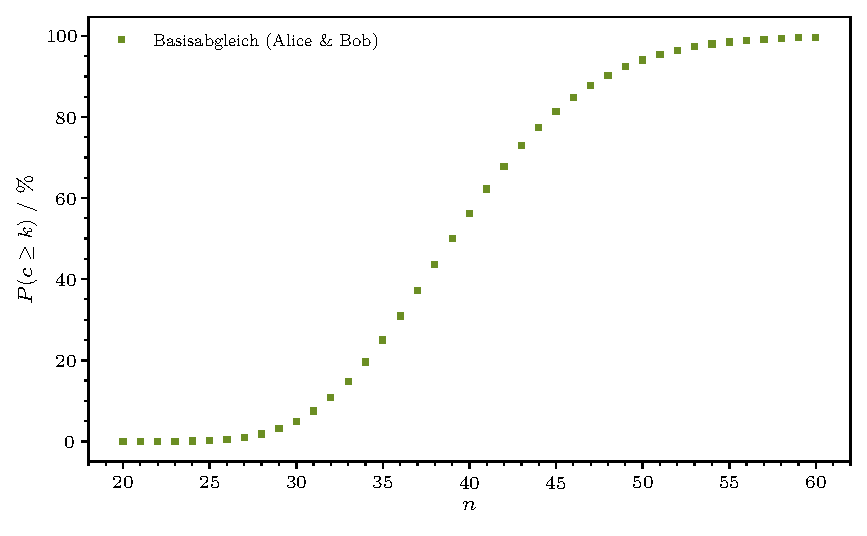
\includegraphics{build/kumuliert.pdf}
	\caption{.}
	\label{fig:kumuliert}
\end{figure}

\qty{96.48}{\percent}

\subsection{Verschlüsselung einer Nachricht}

\begin{longtable}[c]{rccrcc}
	\caption{.}
	\label{tab:schluessel}
	\\
	\expandableinput{content/tabelle/schluessel.tex}
\end{longtable}

\qty{7.84}{\percent}

\begin{table}[H]
	\centering
	\caption{.}
	\label{tab:alice}
	\begin{tabular}{lcccc}
		\expandableinput{content/tabelle/alice.tex}
	\end{tabular}
\end{table}

\begin{table}[H]
	\centering
	\caption{.}
	\label{tab:bob}
	\begin{tabular}{lcccc}
		\expandableinput{content/tabelle/bob.tex}
	\end{tabular}
\end{table}

\subsection{Identifikation eines Abhörversuchs}

\begin{longtable}[c]{rccrccc}
	\caption{.}
	\label{tab:abhoeren}
	\\
	\expandableinput{content/tabelle/abhoeren.tex}
\end{longtable}

\begin{figure}[H]
	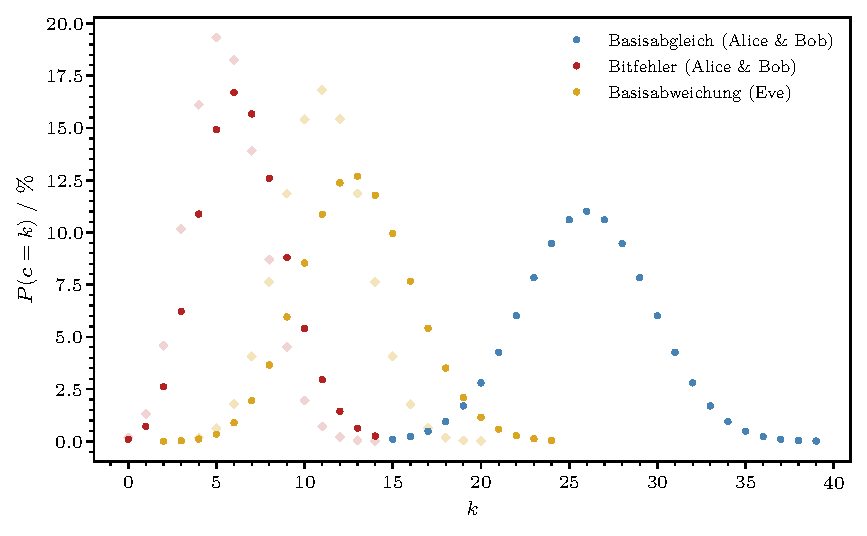
\includegraphics{build/verteilung.pdf}
	\caption{.}
	\label{fig:verteilung}
\end{figure}

\qty{6.01}{\percent}

\qty{10.86}{\percent}

\qty{10.88}{\percent}

\qty{16.82}{\percent}

\qty{16.11}{\percent}
